\clearpage
\section{Ableitungstabelle}

\begin{center}
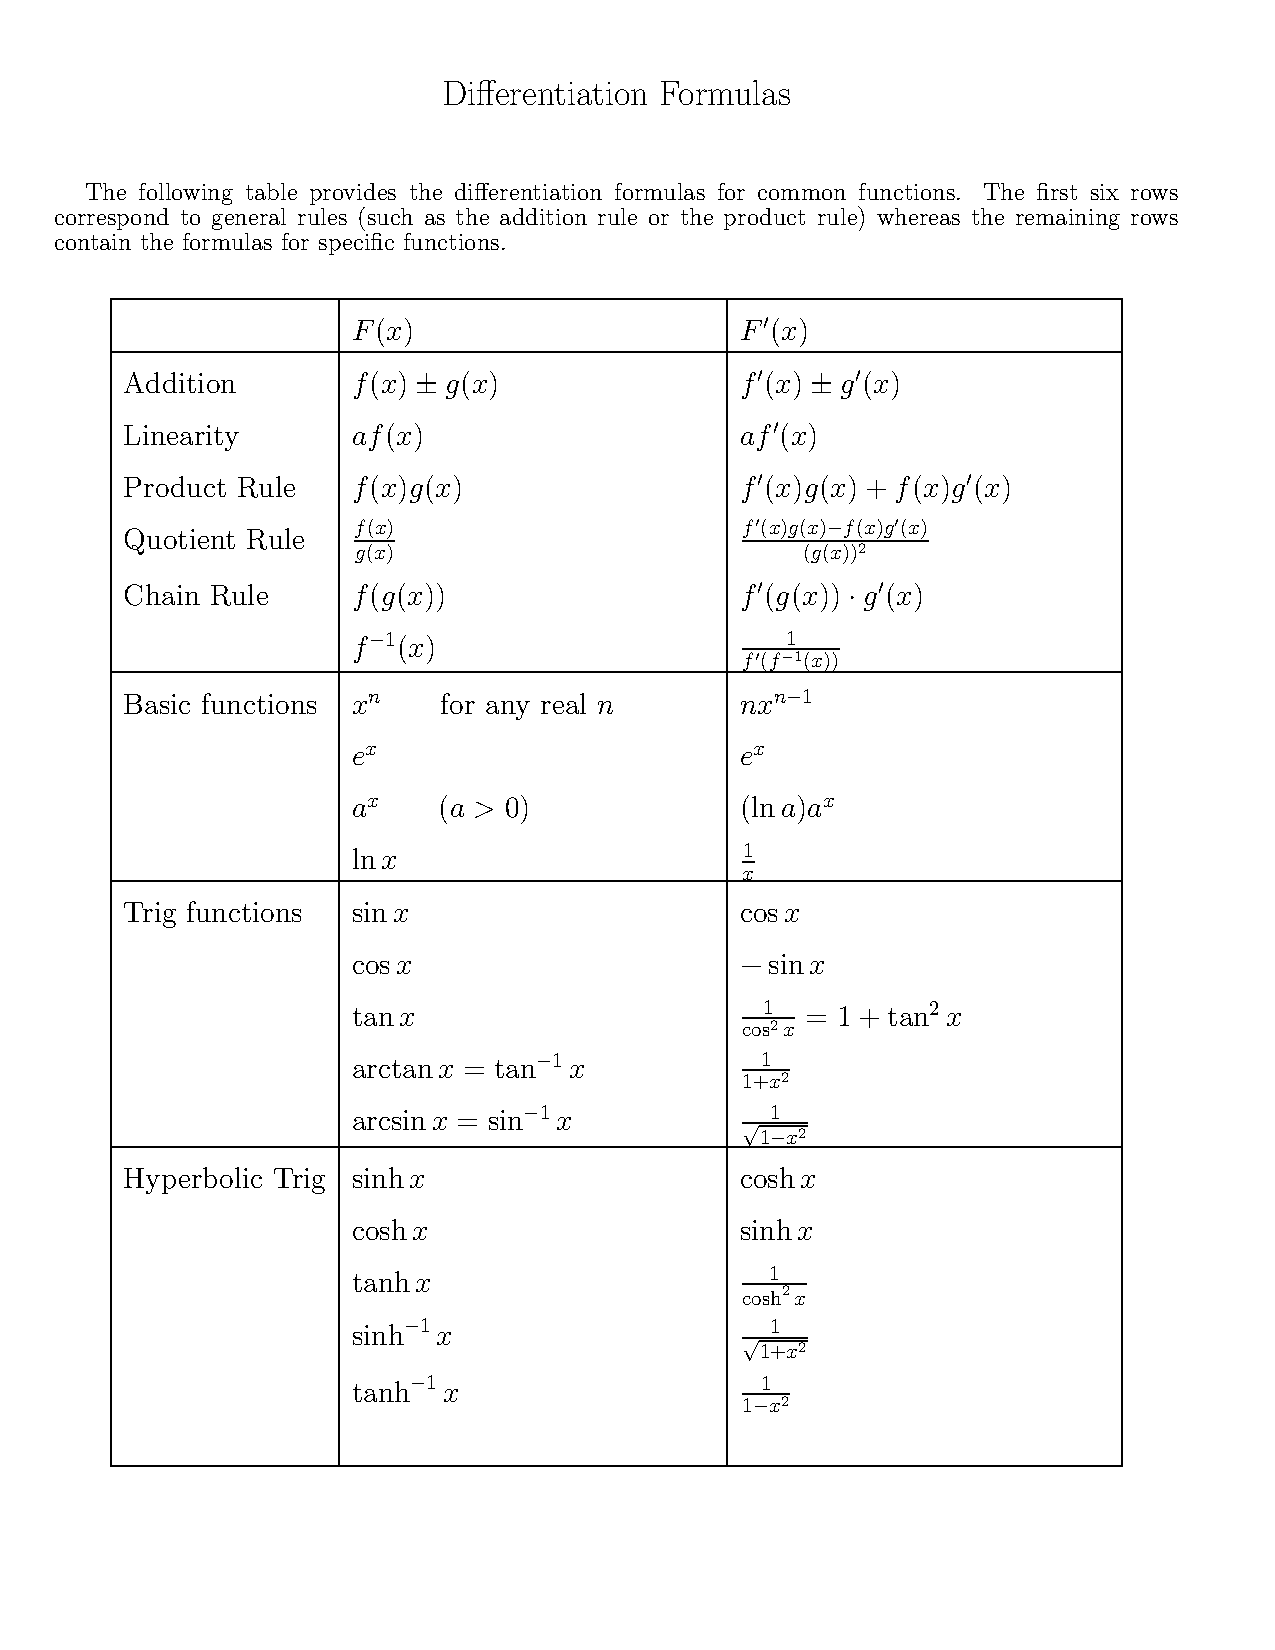
\includegraphics[page=1,width=14cm,trim=1.75cm 3.0cm 2.5cm 5.0cm,clip]{./files/calcrulz.pdf}
%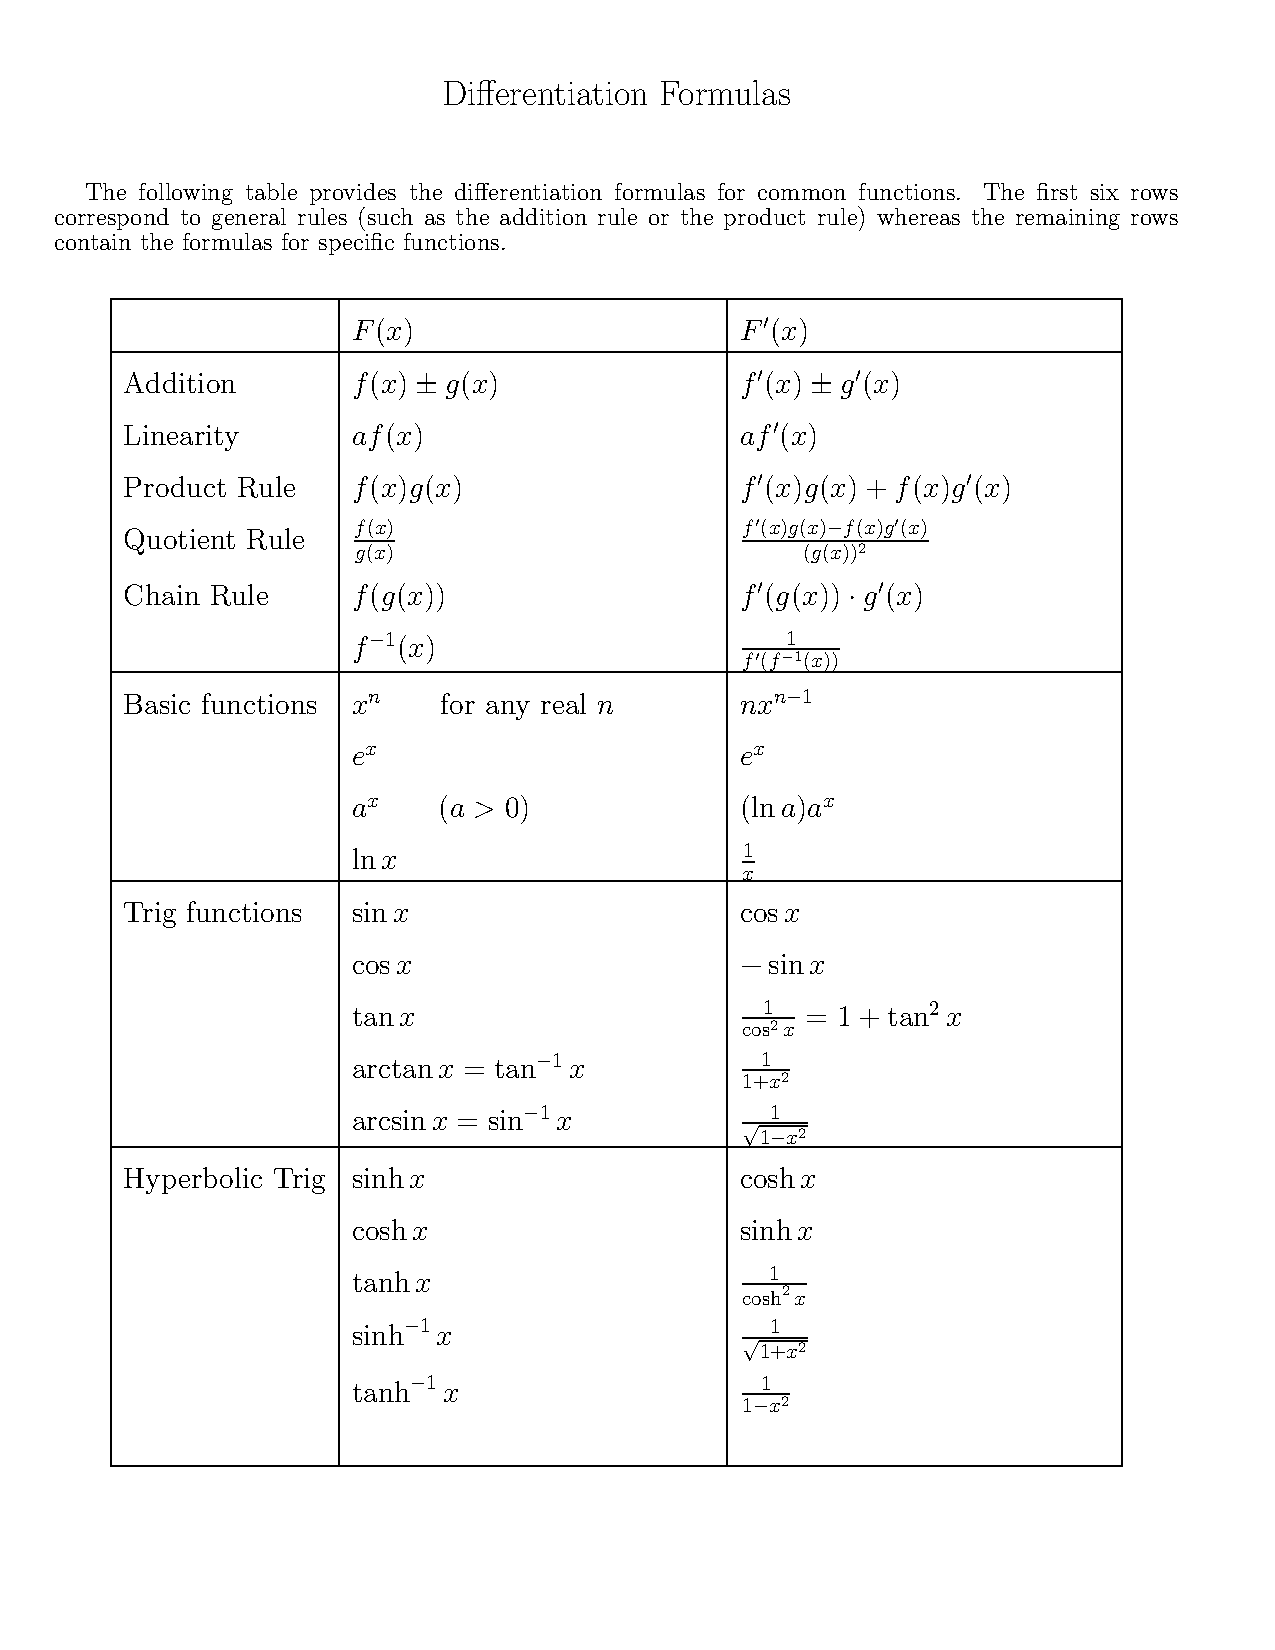
\includegraphics[page=1,width=14cm,clip]{./files/calcrulz.pdf}
\end{center}
\hfill
\section{Übersicht der Polynome}
\begin{tabular}{l|lll}
Name & Formel & Beispiel & Referenz \\
\hline
Newton    & $\pi_n(x) =\prod_{i=1}^n(x-x_{i-1})$  & $\pi_2=(x-x_0)(x-x_1)$ & \ref{ssec:newton_polynom}, S.~\pageref{ssec:newton_polynom}\\
Bernstein & $B_{i,n}(x)=\binom{n}{i}(1-x)^{n-i} x^i$   & $B_{1,2}=2x(1-x)$ & \ref{sssec:spline_bernsteinpoly}, S.~\pageref{sssec:spline_bernsteinpoly} \\
Monomials & $x^n$                       & $x^2$ & \ref{sssec:ls_monomiale}, S.~\pageref{sssec:ls_monomiale} \\
Orthogonale & $p_{k,N}(t) = \sum\limits_{i=0}^k (-1)^i \binom{k}{i} \binom{k+i}{i} \frac{t^{(i)}}{N^{(i)}}$ & $P_1(x)=1-\frac{x-3}{2}$ & \ref{sssec:ls_orthogonal}, S.~\pageref{sssec:ls_orthogonal} \\
Chebyshev & $T_n(x)=\cos(n \arccos(x))$ & $T_2=2x^2-1$ & \ref{sssec:chebyshev_polynom}, S.~\pageref{sssec:chebyshev_polynom} \\


\end{tabular}
\newpage

\section{Integrationstabelle}

\begin{center}
\includegraphics[page=2,width=18cm,trim=1.25cm 3cm 4.5cm 4cm,clip]{./files/calcrulz.pdf}
%\includegraphics[page=2,width=18cm,clip]{./files/calcrulz.pdf}
\end{center}
